\documentclass[10pt]{beamer}
\usetheme{Madrid}
\usepackage{booktabs}
\usepackage{graphicx}
\usepackage[T1]{fontenc}
\usepackage{tikz}
\usetikzlibrary{arrows.meta}
\setbeamertemplate{navigation symbols}{}
% To view speaker notes, uncomment the next line (adds note pages):
% \setbeameroption{show notes}
\tikzset{
  box/.style={draw, rounded corners, align=center, text width=2.3cm, minimum height=0.9cm, font=\scriptsize},
  kuser/.style={box, fill=blue!15}, kagent/.style={box, fill=green!25},
  kdata/.style={box, fill=black!8}, kdanger/.style={box, fill=red!25},
  koutput/.style={box, fill=orange!25}, kdecision/.style={box, fill=yellow!30},
  kguard/.style={box, fill=violet!25},
  flow/.style={-{Stealth[length=2mm]}, thick},
}
% ======================= EDIT YOUR DETAILS =======================
\newcommand{\studentname}{Aflah Muhammed P}
% Change the university roll/registration number:
\newcommand{\rollno}{TVE23CSXXX}
% Change your class roll number:
\newcommand{\rollclass}{Roll No: XX}
% Change your guide name:
\newcommand{\guidename}{Prof. Guide Name}
% Change department / college / short-institute if needed:
\newcommand{\deptname}{Department of Computer Science and Engineering}
\newcommand{\collegename}{College of Engineering Trivandrum}
\newcommand{\shortinst}{CET}
% Change the seminar date:
\newcommand{\seminardate}{\today}
% =================================================================
\title[B.Tech Seminar]{Teamwork for AI: How LLM Agents Collaborate to Solve Big Problems}
\subtitle{Based on: Multi-Agent Collaboration Mechanisms: A Survey of LLMs (arXiv:2501.06322, 2025)}
\author[\studentname\ (\shortinst)]{\studentname \\ \small \rollno \\ \small \rollclass \\ \small Guide: \guidename}
\institute[]{\deptname \\ \collegename}
\date{\seminardate}
\begin{document}
\begin{frame}[plain]
  \titlepage
\end{frame}
\begin{frame}{Table of Contents}
  \tableofcontents
\end{frame}
\section{Introduction}
\begin{frame}{Introduction}
\begin{itemize}
  \item A single LLM is powerful but limited on large, multi-step tasks.
  \item Multi-agent systems let several LLM agents work together like a team.
  \item Each agent has a role, its own memory, tools, and a shared goal.
  \item This survey maps how agents talk, coordinate, and combine answers.
  \item It gives beginners a shared vocabulary for building agent teams.
  \item Real uses span 5G/6G networks, Industry 5.0, and question answering.
\end{itemize}
\end{frame}
\note{Welcome everyone. Today we are looking at how several AI agents can team up to solve problems that are too big for one model alone. Think of it as moving from a single expert to a whole project team, where each member has a job. By the end you will have the vocabulary to describe how these agent teams actually work.}
\section{Literature Survey}
\begin{frame}{Literature Survey / Background}
  \small
  \begin{tabular}{@{}p{2.7cm}p{2.3cm}p{5.6cm}@{}}
    \toprule
    \textbf{Title} & \textbf{Author} & \textbf{Summary} \\
    \midrule
    A Survey on LLM-based Autonomous Agents & Wang et al., 2024 & Reviews single-agent design (profile, memory, planning, action), the building blocks later reused inside agent teams. \\
    \addlinespace
    CAMEL: Communicative Agents & Li et al., 2023 & Introduces role-playing agents that cooperate through structured conversation to finish tasks with little human input. \\
    \addlinespace
    AutoGen: Multi-Agent Conversation Framework & Wu et al., 2023 & Open framework letting developers compose conversable agents with flexible, customizable communication and coordination patterns. \\
    \addlinespace
    \bottomrule
  \end{tabular}
\end{frame}
\note{Before this survey, a few key works set the stage. One line of research described how to build a single autonomous agent from an LLM. Others, like CAMEL and AutoGen, showed agents talking to each other to get work done. This paper builds on all of them by giving one common framework.}
\section{Motivation}
\begin{frame}{Motivation}
\begin{itemize}
  \item Complex real tasks exceed what one prompt or model can handle.
  \item Splitting work across specialist agents improves reasoning and accuracy.
  \item Debate and review between agents catch mistakes a solo model misses.
  \item The field lacked a shared language for how agents collaborate.
  \item A clear framework helps beginners and researchers compare systems.
\end{itemize}
\end{frame}
\note{Why do we need this? A single prompt struggles with long, complicated tasks that have many steps. When you split the work across specialist agents and let them check each other, you often get better and more reliable answers. But the field was messy, with no shared way to describe these setups, and that is the gap this paper fills.}
\section{Problem Statement}
\begin{frame}{Problem Statement}
  \begin{block}{}
  There was no unified vocabulary or framework for describing how LLM agents actually collaborate, making systems hard to compare, design, and improve. This survey defines collaboration mechanisms so agent teams can be reasoned about systematically.
  \end{block}
\end{frame}
\note{The core problem is simple: everyone was building agent teams differently, with no common language to describe them. That makes systems hard to compare or improve. So the authors set out to define exactly what a collaboration mechanism is.}
\section{Objectives}
\begin{frame}{Objectives}
\begin{itemize}
  \item Define LLM-based agents and multi-agent systems in plain terms.
  \item Introduce a collaboration framework built on five key dimensions.
  \item Explain cooperation, competition, and coopetition among agents.
  \item Compare communication structures and coordination strategies.
  \item Survey real applications in networking, industry, and question answering.
  \item Identify open challenges and promising future research directions.
\end{itemize}
\end{frame}
\note{The paper has a few clear goals. First, define agents and multi-agent systems plainly. Then introduce a five-part framework for collaboration, explain the ways agents interact, and finally survey where this is used in the real world and what is still unsolved.}
\section{Methodology}
\begin{frame}[allowframebreaks]{Methodology: Defining the Agent and the System}
\begin{itemize}
  \item An agent is an LLM plus a role, memory, and tools.
  \item The paper formally writes an agent as elements m, o, e, x, y.
  \item m is the model, o its objective, e its environment.
  \item x is the input it perceives; y is the action it outputs.
  \item Many agents joined by channels form a multi-agent system.
\end{itemize}
\end{frame}
\note{Their approach has three parts. First they formally define a single agent as a model with an objective, an environment, inputs, and outputs. Then they describe the collaboration channel using five dimensions. Finally they use those dimensions to classify existing systems and applications. Do not worry about the symbols; the idea is just a tidy checklist for describing any agent team.}
\begin{frame}[allowframebreaks]{Methodology: The Collaboration Channel: Five Dimensions}
\begin{itemize}
  \item Actors: which agents take part in the interaction.
  \item Types: cooperation, competition, or coopetition between agents.
  \item Structures: peer-to-peer, centralized, distributed, or hierarchical.
  \item Strategies: rule-based, role-based, or model-based control.
  \item Coordination: protocols for when and how agents exchange messages.
\end{itemize}
\end{frame}
\begin{frame}[allowframebreaks]{Methodology: Surveying Mechanisms and Applications}
\begin{itemize}
  \item Classify existing systems using the five dimensions.
  \item Map frameworks like AutoGen, MetaGPT, and CAMEL onto the taxonomy.
  \item Review domains: 5G/6G, Industry 5.0, QA, and social settings.
  \item Extract lessons, open challenges, and research directions.
\end{itemize}
\end{frame}
\section{Key Concepts}
\begin{frame}[allowframebreaks]{Key Concepts}
  \begin{description}
    \item[LLM agent] An LLM given a role, memory, and tools to perceive and act toward a goal.
    \item[Multi-agent system (MAS)] Several agents coordinating through channels to solve a task collectively.
    \item[Collaboration channel] The link connecting agents, described by five dimensions.
    \item[Cooperation] Agents align objectives and work together toward one shared goal.
    \item[Competition] Agents pursue their own goals, for example debating opposing sides.
    \item[Coopetition] Agents cooperate on some parts while competing on others.
  \end{description}
\end{frame}
\note{Let us lock in the vocabulary. An agent is an LLM given a role, memory, and tools. A multi-agent system is several of these working together. The interaction can be cooperation, competition, or a mix called coopetition. Keep these words in mind, because the whole paper is organized around them.}
\section{System Architecture}
\begin{frame}{System Architecture}
  \begin{center}
  \resizebox{0.96\textwidth}{!}{%
  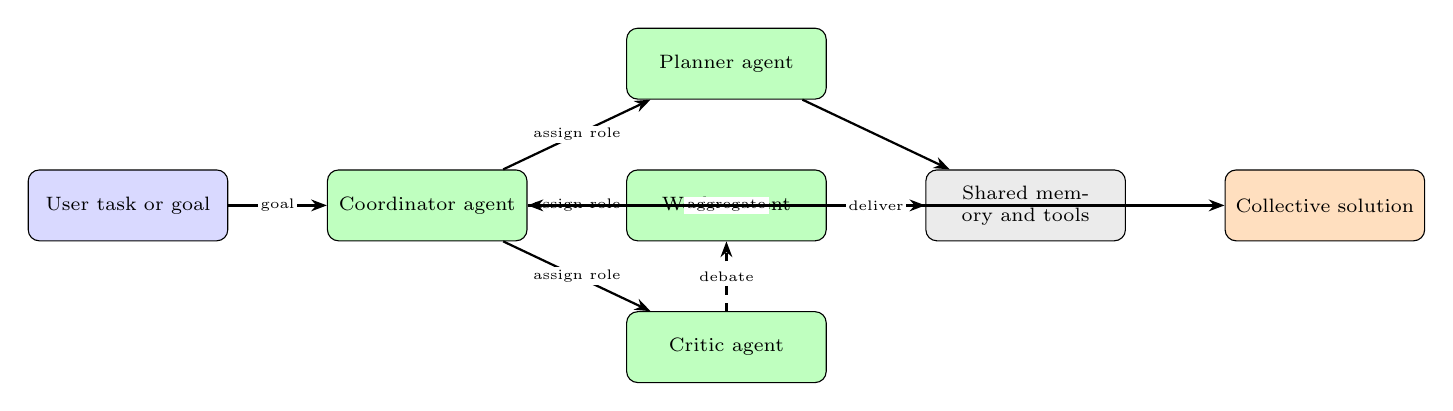
\begin{tikzpicture}
    \node[kuser] (user) at (0.00,0.00) {User task or goal};
    \node[kagent] (coord) at (3.80,0.00) {Coordinator agent};
    \node[kagent] (planner) at (7.60,1.80) {Planner agent};
    \node[kagent] (coder) at (7.60,0.00) {Worker agent};
    \node[kagent] (critic) at (7.60,-1.80) {Critic agent};
    \node[kdata] (memory) at (11.40,0.00) {Shared memory and tools};
    \node[koutput] (output) at (15.20,0.00) {Collective solution};
    \draw[flow] (user) -- (coord) node[midway, font=\tiny, fill=white, inner sep=1pt]{goal};
    \draw[flow] (coord) -- (planner) node[midway, font=\tiny, fill=white, inner sep=1pt]{assign role};
    \draw[flow] (coord) -- (coder) node[midway, font=\tiny, fill=white, inner sep=1pt]{assign role};
    \draw[flow] (coord) -- (critic) node[midway, font=\tiny, fill=white, inner sep=1pt]{assign role};
    \draw[flow] (planner) -- (memory);
    \draw[flow] (coder) -- (memory);
    \draw[flow, dashed] (critic) -- (coder) node[midway, font=\tiny, fill=white, inner sep=1pt]{debate};
    \draw[flow] (memory) -- (coord) node[midway, font=\tiny, fill=white, inner sep=1pt]{aggregate};
    \draw[flow] (coord) -- (output) node[midway, font=\tiny, fill=white, inner sep=1pt]{deliver};
  \end{tikzpicture}%
  }
  \end{center}
  \begin{center}\scriptsize A coordinator assigns roles to specialist agents that share memory and debate to build a collective solution.\end{center}
\end{frame}
\note{Here is the big picture on screen. A user hands a goal to a coordinator agent, which assigns roles to specialist agents. Those agents read and write to a shared memory and use tools, and a critic agent gives feedback to improve the work. Finally the coordinator combines everything into one solution. Follow the arrows left to right and you have the whole loop.}
\begin{frame}[allowframebreaks]{How It Works (Explained)}
\begin{itemize}
  \item A user submits a task or goal to the system.
  \item A coordinator agent receives it and assigns specialist roles.
  \item Planner, worker, and critic agents each handle part of the work.
  \item Agents read from and write to shared memory and external tools.
  \item The critic debates and gives feedback to workers, refining answers.
  \item The coordinator aggregates results and delivers the collective solution.
\end{itemize}
\end{frame}
\section{Example Walkthrough}
\begin{frame}[allowframebreaks]{Example Walkthrough: Example: Building a Small App with an Agent Team}
\begin{enumerate}
  \item User asks the system to build a simple to-do list web app.
  \item Coordinator agent splits the job and assigns roles.
  \item Planner agent writes a step-by-step design and file list.
  \item Coder agent writes the code and saves it to shared memory.
  \item Critic agent reviews the code and flags a bug.
  \item Coder agent fixes the bug using the critic's feedback.
  \item Coordinator combines the pieces and returns the finished app.
\end{enumerate}
\end{frame}
\note{Let us make it concrete with a simple example: building a to-do list app. The coordinator splits the task, the planner designs it, the coder writes it, and the critic finds a bug. The coder fixes it, and the coordinator returns the finished app. Notice how each agent does one job and they pass work between them, just like a real team.}
\section{Results}
\begin{frame}[allowframebreaks]{Results / Findings}
\begin{itemize}
  \item The framework defines 5 core dimensions of every collaboration channel.
  \item It names 3 interaction types: cooperation, competition, and coopetition.
  \item It distinguishes 3 strategies: rule-based, role-based, and model-based.
  \item It surveys 4 application domains: 5G/6G, Industry 5.0, QA, and social.
  \item Written by 6 authors and released on arXiv on 10 January 2025.
  \item It is a conceptual survey: the contribution is the taxonomy, not benchmark scores.
\end{itemize}
\end{frame}
\note{Now, this is a survey, not an experiment, so the results are the framework itself. The headline is five dimensions for any collaboration channel, three types of interaction, three control strategies, and four application areas. Six authors published it on arXiv in January 2025. So when I say results, I mean the organizing map they give us, not benchmark scores.}
\section{Discussion}
\begin{frame}{Discussion}
\begin{itemize}
  \item A shared vocabulary makes agent systems easier to design and compare.
  \item Coopetition, such as debate, can raise answer quality and reliability.
  \item Centralized coordinators are simple but can become bottlenecks.
  \item The best structure depends on the task and its cost constraints.
\end{itemize}
\end{frame}
\note{A few takeaways. Having shared vocabulary genuinely helps you design and compare systems. Letting agents debate can raise quality, but a central coordinator can also become a bottleneck. The best structure really depends on your task and your budget.}
\section{Challenges}
\begin{frame}{Limitations \& Challenges}
\begin{itemize}
  \item The survey is conceptual, without experiments comparing the mechanisms.
  \item Rapid field growth means some newer frameworks are already missing.
  \item Agents can cascade errors and hallucinations across many turns.
  \item Standard benchmarks for multi-agent collaboration are still lacking.
\end{itemize}
\end{frame}
\note{Let us be honest about the limits. Because it is conceptual, the paper does not run experiments comparing these mechanisms head to head. The field moves so fast that some new systems are already missing, and agents can still spread errors across many turns. We also lack solid benchmarks for this kind of collaboration.}
\section{Future Work}
\begin{frame}{Future Work}
\begin{itemize}
  \item Build standardized benchmarks to evaluate agent collaboration fairly.
  \item Develop safety, alignment, and trust mechanisms for agent teams.
  \item Improve long-horizon planning and memory across many interactions.
  \item Move toward artificial collective intelligence at larger scale.
\end{itemize}
\end{frame}
\note{Looking ahead, the authors call for standard benchmarks so we can measure agent teams fairly. They want stronger safety and alignment, better long-term planning and memory, and ultimately a step toward what they call artificial collective intelligence.}
\section{Conclusion}
\begin{frame}{Conclusion}
\begin{itemize}
  \item Multi-agent LLM systems shift AI from solo models to teamwork.
  \item Collaboration channels have five dimensions worth learning as vocabulary.
  \item Types, structures, and strategies together shape how agents cooperate.
  \item This framework guides beginners and researchers building future agent teams.
\end{itemize}
\end{frame}
\note{To wrap up: multi-agent LLM systems move us from solo models to teamwork. Remember the five dimensions of a collaboration channel, and the three interaction types. That vocabulary is the real gift of this paper, and it is a great foundation whether you are studying or building agent systems. Thank you.}
\section{References}
\begin{frame}[allowframebreaks]{References}
  \footnotesize
  \begin{enumerate}
    \item Tran, K.-T., Dao, D., Nguyen, M.-D., Pham, Q.-V., O'Sullivan, B., \& Nguyen, H. D. (2025). Multi-Agent Collaboration Mechanisms: A Survey of LLMs. arXiv:2501.06322.
    \item Wang, L., et al. (2024). A Survey on Large Language Model based Autonomous Agents. Frontiers of Computer Science, 18(6).
    \item Li, G., Hammoud, H., Itani, H., Khizbullin, D., \& Ghanem, B. (2023). CAMEL: Communicative Agents for Mind Exploration of Large Scale Language Model Society. NeurIPS 2023.
    \item Wu, Q., et al. (2023). AutoGen: Enabling Next-Gen LLM Applications via Multi-Agent Conversation. arXiv:2308.08155.
    \item Hong, S., et al. (2023). MetaGPT: Meta Programming for a Multi-Agent Collaborative Framework. arXiv:2308.00352.
    \item Park, J. S., et al. (2023). Generative Agents: Interactive Simulacra of Human Behavior. ACM UIST 2023.
  \end{enumerate}
\end{frame}
\begin{frame}[plain]
  \begin{center}
    {\Huge Thank You}\\[1em]
    {\large Questions?}
  \end{center}
\end{frame}
\end{document}